%%%%%%%%%%%%%%%%%%%%%%%%%%%%%%%%%%%%%%%%%
% Beamer Presentation
% LaTeX Template
% Version 1.0 (10/11/12)
%
% This template has been downloaded from:
% http://www.LaTeXTemplates.com
%
% License:
% CC BY-NC-SA 3.0 (http://creativecommons.org/licenses/by-nc-sa/3.0/)
%
%%%%%%%%%%%%%%%%%%%%%%%%%%%%%%%%%%%%%%%%%

%----------------------------------------------------------------------------------------
%	PACKAGES AND THEMES
%----------------------------------------------------------------------------------------

\documentclass{beamer}

\mode<presentation> {

% The Beamer class comes with a number of default slide themes
% which change the colors and layouts of slides. Below this is a list
% of all the themes, uncomment each in turn to see what they look like.

%\usetheme{default}
%\usetheme{AnnArbor}
%\usetheme{Antibes}
%\usetheme{Bergen}
%\usetheme{Berkeley}
%\usetheme{Berlin}
%\usetheme{Boadilla}
%\usetheme{CambridgeUS}
%\usetheme{Copenhagen}
%\usetheme{Darmstadt}
%\usetheme{Dresden}
%\usetheme{Frankfurt}
%\usetheme{Goettingen}
%\usetheme{Hannover}
%\usetheme{Ilmenau}
%\usetheme{JuanLesPins}
%\usetheme{Luebeck}
\usetheme{Madrid}
%\usetheme{Malmoe}
%\usetheme{Marburg}
%\usetheme{Montpellier}
%\usetheme{PaloAlto}
%\usetheme{Pittsburgh}
%\usetheme{Rochester}
%\usetheme{Singapore}
%\usetheme{Szeged}
%\usetheme{Warsaw}

% As well as themes, the Beamer class has a number of color themes
% for any slide theme. Uncomment each of these in turn to see how it
% changes the colors of your current slide theme.

%\usecolortheme{albatross}
%\usecolortheme{beaver}
%\usecolortheme{beetle}
%\usecolortheme{crane}
%\usecolortheme{dolphin}
%\usecolortheme{dove}
%\usecolortheme{fly}
%\usecolortheme{lily}
%\usecolortheme{orchid}
%\usecolortheme{rose}
%\usecolortheme{seagull}
%\usecolortheme{seahorse}
%\usecolortheme{whale}
%\usecolortheme{wolverine}

%\setbeamertemplate{footline} % To remove the footer line in all slides uncomment this line
%\setbeamertemplate{footline}[page number] % To replace the footer line in all slides with a simple slide count uncomment this line

%\setbeamertemplate{navigation symbols}{} % To remove the navigation symbols from the bottom of all slides uncomment this line
}

\usepackage{graphicx} % Allows including images
\usepackage{booktabs} % Allows the use of \toprule, \midrule and \bottomrule in tables

%----------------------------------------------------------------------------------------
%	TITLE PAGE
%----------------------------------------------------------------------------------------

\title[GenerAL]{A Review of Generative Attention Learning} % The short title appears at the bottom of every slide, the full title is only on the title page

\author{Jaime Canizales} % Your name
\institute[Hunter College] % Your institution as it will appear on the bottom of every slide, may be shorthand to save space
{
City University of New York \\ % Your institution for the title page
\medskip
\textit{jaime.canizales@hunter.cuny.edu} % Your email address
}
\date{\today} % Date, can be changed to a custom date

\begin{document}

\begin{frame}
\titlepage % Print the title page as the first slide
\end{frame}
\begin{frame}
\frametitle{Overview} % Table of contents slide, comment this block out to remove it
\tableofcontents % Throughout your presentation, if you choose to use \section{} and \subsection{} commands, these will automatically be printed on this slide as an overview of your presentation
\end{frame}

\section{Introduction}


\begin{frame}\frametitle{Introduction} 
\begin{block}{Problem Statement}
How to solve the problem of \textbf{smartly} grasping(e.g., grabbing a pitcher by the handle) an object in a cluttered real world environment, using a high degree of freedom(DOF) robot hand(up to 6 degrees) not restricted to any particular camera view or grasping strategy to simplify the problem(e.g., top down grasps, where the robot hand acts as a claw machine and grabs the object from above).
\end{block}

\end{frame}

%----------------------------------------------------------------------------------------
%	PRESENTATION SLIDES
%----------------------------------------------------------------------------------------

\begin{frame}\frametitle{Introduction(cont.)} 
\begin{block}{Solution proposed in paper}
Using a reinforcement learning framework, which takes a single depth image as input; we can find the end-effector position and orientation, as well as a set of finger joint angles in a timely manner(close to real time).
\end{block}
\end{frame}    

\begin{frame}{Why is this hard?}
\begin{itemize}
\item As the DOF increases in a robot hand, the training data needed to find a reliable solutions increases exponentially. 
\item Real world problems must inherently deal with cartesian spaces as their solution spaces(Finding solutions is difficult in cartesian spaces, because the spaces are infinite, continuous and the number of possible solutions may be infinite).   
\end{itemize}
\end{frame}

\begin{frame}{Why is this hard?(cont.)}
\begin{itemize} 
\item Not restricted to only top-down grasping solutions(top-down grasping solutions decrease the complexity of the problem in two ways: End-effector position and orientation solution is simplified from $\mathbb{R}^6$ to $\mathbb{R}^4$, constraints are added to solution space decreasing complexity ).
\item slight perturbations of a good solution can lead to bad solutions.
\end{itemize}
\end{frame}

\begin{frame}{Alleviating these complexities}
\begin{itemize}
\item Uses a deep convolutional Reinforcement learning(RL) framework to solve the problem in reasonable time.
\item Trained in simulation but used in the real world.
\item A zooming mechanism is applied to objects to optimize good grasps.
\item Action space, states, and RL policies are all learned and optimized in pixel space(smaller and discrete).
\end{itemize}
\end{frame}

\section{Technical Information}
\begin{frame}{Technical Information}
\begin{itemize}
\item Uses an infinite horizon Partially Observable Markov Decision Process(POMDP), because agent(robot) can't observe rgb info, and the complete 3D geometry of objects and scene.
\item infinite horizon(no clear start or end state) implies the magnitude for the set of instructions to achieve goal is unknown [$\pi_1,\pi_2,\pi_3,\pi_4,...$]=$\pi$ (policy).  
\end{itemize}  
\end{frame}

\begin{frame}{POMDP}
\begin{itemize}
\item Six tuple definition $<$S, A,$\rho_0$,R,T, $\gamma$ $>$
\item observation space S - states of the agent(robot) in the environment(observations).
\item Action space A - set of actions that can be performed by the agent.
\item $\rho_0$ initial state distribution $\rho_0 \in \Pi(\text{S})$ - initial probability of being in any given state(randomly initialized).
\item Dynamics model T: S $\times$ A $\rightarrow \Pi(\text{S})$ - for all state-action pairs, return the probabilities of going to the next states.
\item $\gamma$ is discount factor $\in [0,1]$ - used more as a hyper parameter to help convergence in infinite horizon POMDP.
\item Reward function R: S $\times$ A $\rightarrow \mathbb{R}$ - Binary indicator function. 1 for successful grasp and 0 otherwise.
\end{itemize}
\end{frame}

\begin{frame}{POMDP(cont.)}
\begin{itemize}
\item The agent acts according to stationary stochastic policies($\pi$ does not change over time) $\pi$ : S $\rightarrow \Pi$(A), which specify action choice probabilities for each observation.
\item Each policy $\pi$ has a corresponding $Q_\pi$ : S $\times$ A $\rightarrow\mathbb{R}$, function that defines the expected discounted cumulative reward for taking action a from observation S and following the policy $\pi$ from that point
onward.\\ $\sum_t \gamma^{t-1} r_t$
\end{itemize}
\end{frame}

\begin{frame}\frametitle{Policy Gradient} 
\begin{block}{Policy Gradient}
Policy gradient methods are a type of RL techniques that rely upon optimizing parameterized policies w.r.t. expected return(long term cumulative reward) by gradient descent.
\end{block}
\begin{block}{Soft proximal policy optimization(SPPO)}
The policy gradient method used in this paper, which follows the formula: $maximize_\theta \text{ }L\text{ }  = \mathbb{E}_{\pi_\theta} [\pi_{\theta} (a_t | S_t)Q_{\pi_\theta} (S_t, a_t)]$ ($\theta$ is the network weights, t is the time step)
\end{block}
\begin{block}{SPPO modifications}
SPPO modified to use Clipped Surrogate Objective (Schulman et al. 2017) and apply a soft advantage target to balance between exploration and exploitation (Haarnoja et al. 2018).
\end{block}

\end{frame}

\begin{frame}\frametitle{Hyper Parameters}
\begin{figure}
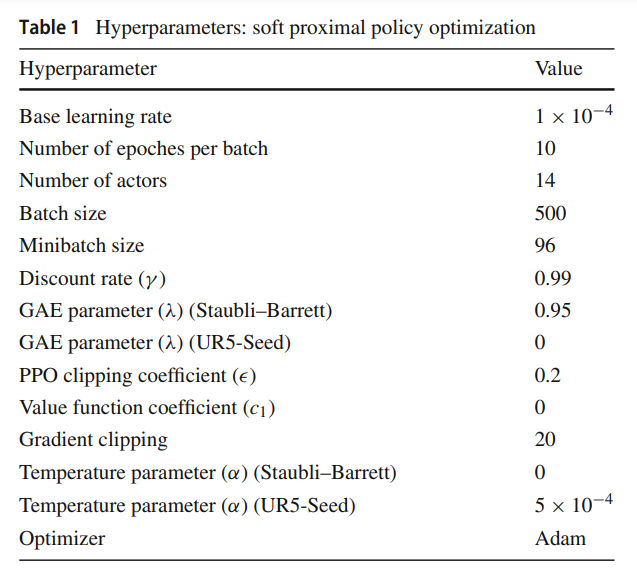
\includegraphics[width=0.5\linewidth]{hyper_parameters}
\end{figure}
\end{frame}

\begin{frame}\frametitle{Learning attention}
\begin{itemize}
\item Decide whether the robot should zoom into the depth map or start grasping. 
\item Determine the level of zooming(scale)(end-effector as center of zoomed image).
\end{itemize}
\end{frame}

\begin{frame}\frametitle{Architecture}
\begin{figure}
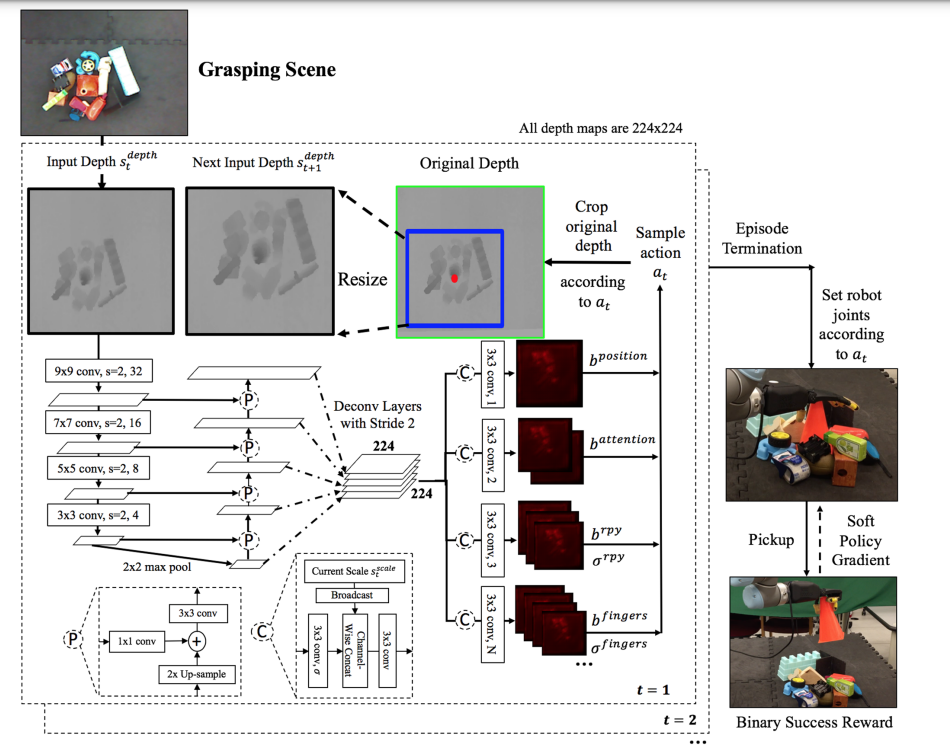
\includegraphics[width=0.8\linewidth]{generAL_architecture}
\end{figure}
\end{frame}

\begin{frame}\frametitle{Architecture(Cont.)}
\begin{itemize}
    \item A feature four branch pyramid branch CNN.
    \item The “P” blocks indicate feature pyramid blocks, giving scale invariance capability to the CNN.
    \item The “C” blocks indicate how GenerAL introduces the current zoom level into each branch.
    \item All convolutional layers have ReLU activations and strides of 1.
    \item Each red-black map proposes pixel-wise grasp configurations and their probabilities.
\end{itemize}
\end{frame}


\begin{frame}\frametitle{Training}
\begin{itemize}
    \item GenerAL is trained entirely in simulation.
    \item During training, a single seen object or a cluttered scene of multiple seen objects is loaded with equal probability.
    \item Random number of objects from 2 to 30 for a simulated cluttered scene.
    \item The number of training grasp attempts required to reach convergence range from 5000 to 15,000.
    \item 24 hour training time on one gpu, 13 virtual cpu machine.
\end{itemize}
\end{frame}

\begin{frame}\frametitle{Testing}
\begin{itemize}
\item GenerAL is tested both in simulation and real-world. Using the ShapeNet Repository in simulation.
\item 200 + seen objects from the YCB and KIT datasets.
\item 100+ novel objects from the BigBIRD dataset.
\item Evaluated 500 grasp attempts per experiment in simulation.
\end{itemize}
\end{frame}

\begin{frame}\frametitle{Performance}
\begin{figure}
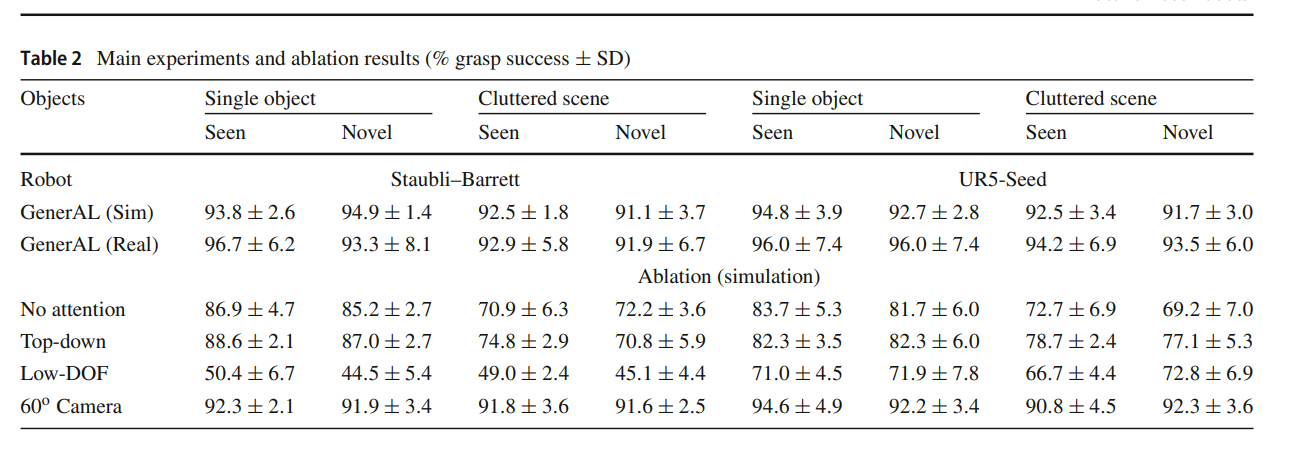
\includegraphics[width=0.8\linewidth]{results}
\end{figure}
\end{frame}

\section{Conclusions and possible extensions}
% \begin{frame}\frametitle{Other Nets}
% \begin{itemize}
%     \item 
% \end{itemize}
% \end{frame}

\begin{frame}\frametitle{possible extensions}
\begin{itemize}
\item By adding segmentation you can accomplish object specific grasping.
\item Solve for collision avoidance.
\end{itemize}
\end{frame}

\begin{frame}
\frametitle{References}
\footnotesize{
\begin{thebibliography}{99} % Beamer does not support BibTeX so references must be inserted manually as below
\bibitem[Wu, 2020]{p1} Bohan Wu,  Iretiayo Akinola,  Abhi Gupta,  Feng Xu,  Jacob Varley,  David Watkins-Valls, and Peter K. Allen (2020)
\newblock Generative Attention Learning: a “GenerAL” framework for
high-performance multi-fingered grasping in clutter
\newblock \emph{© Springer Science+Business Media, LLC, part of Springer Nature 2020}.

\bibitem[Zhou, 2018]{p2} Haarnoja, T., Zhou, A., Abbeel, P., and Levine, S. (2018)
\newblock Soft actor-critic: Off-policy maximum entropy deep reinforcement learning with a stochastic actor.
\newblock \emph{International conference on machine learning(ICML)}.

\bibitem[Schulman, 2017]{p3} Schulman, J., Wolski, F., Dhariwal, P., Radford, A., and  Klimov, O. (2017).
\newblock Proximal policy optimization algorithms. 
\newblock \emph{arXiv preprint}
\end{thebibliography}
}
\end{frame}


%https://www.cs.columbia.edu/~allen/PAPERS/General_Auro_2020.pdf


\end{document}